% Provenance (never printed): old terminale S material on the disappearance of
% mountain ranges (erosion, transport, sedimentation, isostatic rebound, the
% recycling of continental material). Owner (Sync 0/1): denudation rate,
% sediment load (bed, suspended, dissolved), isostatic rebound, detrital rock,
% diagenesis. Weathering, erosion, deposition are Book 1's (g5); hydrolysis and
% clay minerals g10.07's; discharge g10.08's; isostasy and Airy's model g11.03's;
% sedimentary basin g11.09's; mountain root g12.01's; metamorphism g12.03's;
% half-life is physics' (recalled in prose). Figures: figdata/grade-12/relief_decay.py
% (rates, decay curves, the Varden unconformity from figdata/shared/region.py).
\chapter{पर्वतों का विनाश}\label{ch:g12:destruction-of-mountains}

अंतर्राष्ट्रीय अंतरिक्ष स्टेशन से देखने पर पूर्वी उत्तर अमेरिका के ऐपलेशियन पर्वत
लंबे, गहरे, वनाच्छादित कटकों और पीली खेतिहर घाटियों का एक आकर्षक पैटर्न दिखते हैं;
नीचे की फ़ोटो में उनके \qty{500}{km} से अधिक हैं। कटक चट्टान की कठोर परतें हैं जो
तब कसे हुए \omterm{def:g12:mountain-building:fold}{वलनों} में मुड़ गईं जब अफ़्रीका ने उत्तर अमेरिका को धकेला, कार्बोनिफ़ेरस और पर्मियन
कल्पों में, 250 मिलियन वर्ष से भी पहले। आज उनका सबसे ऊँचा शिखर, माउंट
मिचेल, मिसिसिपी नदी के पूर्व का सबसे ऊँचा बिंदु, समुद्र-तल से
\qty{2037}{m} ऊपर खड़ा है, एवरेस्ट की ऊँचाई के एक-चौथाई से भी कम।
% ledger: photo:g12-appalachians, usgs:alleghanian, usgs:alleghanian-age, ics:base.Triassic, ncparks:mitchell (6684 ft), tht:everest (Book 1 row, 8848.86 m)

\begin{omfigure}
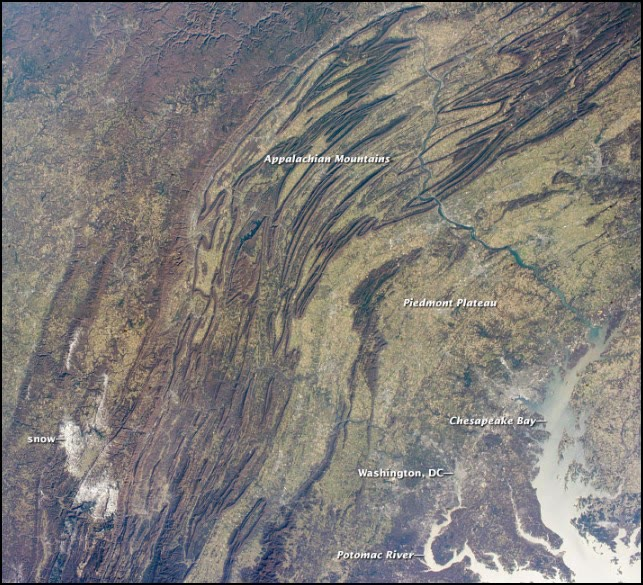
\includegraphics[width=0.6\linewidth]{images/book2/g12-iss-appalachians.jpg}

{\small घाटी-और-कटक वाले ऐपलेशियन, उत्तर-पूर्वी पेन्सिलवेनिया
(ऊपर दाएँ) से वेस्ट वर्जीनिया तक, 17 नवंबर 2012 को अंतर्राष्ट्रीय अंतरिक्ष
स्टेशन से खींचे गए। वनाच्छादित कटक चट्टान की कठोर परतें हैं,
खेतिहर घाटियाँ नरम परतें। फ़ोटो नासा (सार्वजनिक डोमेन)।}
\end{omfigure}
% ledger: photo:g12-appalachians

कोई पर्वत-श्रेणी टिकती नहीं। जिस क्षण वह उठती है, उसी क्षण से वर्षा, बर्फ़ और
नदियाँ उस पर आक्रमण करती हैं; जो चट्टान वे बहा ले जाती हैं, वह समुद्र में पहुँचती है, जहाँ वह
नई चट्टान बनती है। यह अध्याय मापता है कि यह कितनी तेज़ी से होता है, मलबे का
उस स्थान तक अनुसरण करता है जहाँ वह पत्थर बनता है, और दिखाता है कि घिसी जाती
श्रेणी घिसते-घिसते ऊपर क्यों उठती रहती है।

\begin{recall}
अपक्षय चट्टान को वहीं तोड़ता है जहाँ वह खड़ी है; अपरदन मलबे को बहा ले जाता है
और निक्षेपण उसे कहीं और बिछा देता है (पुस्तक 1, कक्षा 5)। \omterm{def:g10:soil-formation:chemical-weathering}{रासायनिक अपक्षय}
\omterm{def:g10:soil-formation:hydrolysis}{जल-अपघटन} द्वारा फ़ेल्डस्पारों को \omterm{def:g10:soil-formation:clay}{मृत्तिका खनिजों} में बदलता है
(\cref{ch:g10:soil-formation})। किसी नदी का \omterm{def:g10:drainage-basins:discharge}{विसर्जन} जल का वह आयतन है
जो एक सेकंड में किसी बिंदु से गुज़रता है (\cref{ch:g10:drainage-basins})।
भूपर्पटी \omterm{def:g11:lithosphere-asthenosphere:isostasy}{समस्थिति} में प्रावार पर तैरती है; एयरी के मॉडल में, जिस क्षेत्र की भूपर्पटी
$\Delta H$ अधिक मोटी है, वह $\Delta H\,(\rho_m - \rho_c)/\rho_m$ अधिक ऊँचा खड़ा होता है
(\cref{ch:g11:lithosphere-asthenosphere}), और ऊँची श्रेणी मोटी भूपर्पटी के एक \omterm{def:g12:continental-crust:root}{मूल}
पर टिकी होती है (\cref{ch:g12:continental-crust})। अवसाद
\omterm{def:g11:fossil-fuel-geology:basin}{अवसादी द्रोणियों} में जमा होते हैं (\cref{ch:g11:fossil-fuel-geology})। किसी पर्वत-पट्टी में
गहरे दबी चट्टानें कायांतरित होती हैं (\cref{ch:g12:metamorphic-rocks})।
\end{recall}

\section{भूमि कितनी तेज़ी से घिसती है?}

\begin{definition}[अनाच्छादन दर]\label{def:g12:destruction-of-mountains:denudation}
किसी क्षेत्र की \emph{अनाच्छादन दर}\index{अनाच्छादन दर} चट्टान की वह माध्य
मोटाई है जो अपक्षय और अपरदन मिलकर उससे प्रति इकाई समय हटाते
हैं। इसे सामान्यतः मीटर प्रति मिलियन वर्ष
(\unit{m/Myr}) में दिया जाता है, जो मिलीमीटर प्रति हज़ार वर्ष के समान है।
\end{definition}
% ledger: pb11:rates (rates in m/Myr), earle:loads

इतनी धीमी चीज़ को कोई कैसे माप सकता है? भूमि से टकराती कॉस्मिक किरणें
चट्टान के सबसे ऊपरी कुछ मीटरों के क्वार्ट्ज़ में एक दुर्लभ समस्थानिक, बेरिलियम-10, बनाती हैं।
कोई सतह जितनी धीमी घिसती है, हर कण शीर्ष के निकट उतनी ही देर रहता है,
और उतना ही अधिक बेरिलियम-10 जमा करता है। किसी नदी की रेत में इसे मापने से
ऊपर की पूरी द्रोणी की माध्य \omterm{def:g12:destruction-of-mountains:denudation}{अनाच्छादन दर} मिलती है, पिछले
हज़ारों से लेकर कई मिलियन वर्षों तक की।
% ledger: pb11:rates (10Be produced within a few metres of the surface; concentration reflects near-surface residence time; 10^3 to 10^6 years)

ऐसे 1599 मापनों के एक संकलन ने पाया कि खुली अनावृत चट्टानें
धीरे-धीरे घिसती हैं, औसतन \qty{12}{m/Myr} (माध्यिका
\qty{5.4}{m/Myr}), और कभी भी \qty{140}{m/Myr} से तेज़ नहीं। पूरी \omterm{def:g10:drainage-basins:drainage-basin}{अपवाह
द्रोणियाँ} कहीं अधिक खोती हैं, औसतन \qty{218}{m/Myr}, पर माध्यिका केवल
\qty{54}{m/Myr} के साथ: कुछ तेज़ द्रोणियाँ माध्य को ऊपर खींच लेती हैं। सबसे तेज़
खड़ी द्रोणियाँ हैं: किसी द्रोणी का माध्य ढाल वह कारक है जो उसकी दर का
सबसे अच्छा पूर्वानुमान देता है। भूकंपीय रूप से सक्रिय प्रदेशों की द्रोणियाँ, जहाँ पर्वत उठ रहे हैं,
शांत प्रदेशों की द्रोणियों से लगभग दुगुनी तेज़ी से अपरदित होती हैं।
% ledger: pb11:rates

\begin{omfigure}
\begin{tikzpicture}
\begin{axis}[omrecord, xbar, xmode=log, log origin=infty, bar width=7pt, bar shift=0pt,
  width=0.62\linewidth, height=6.6cm, scale only axis, xmin=3, xmax=1000,
  ymin=0.4, ymax=10.6, ytick={1,...,10}, y tick label style={font=\scriptsize, align=right},
  yticklabels={{अनावृत चट्टान, माध्यिका}, {अनावृत चट्टान, माध्य}, {संसार की नदियाँ (लेखा)}, {द्रोणियाँ, माध्यिका},
    {मिसिसिपी, 1900 से पहले (लेखा)}, {शुष्क द्रोणियाँ, माध्य}, {शांत द्रोणियाँ, माध्य}, {द्रोणियाँ, माध्य},
    {भूकंपीय रूप से सक्रिय द्रोणियाँ, माध्य}, {ध्रुवीय द्रोणियाँ, माध्य}},
  xlabel={अनाच्छादन दर (\unit{m/Myr}), लघुगणकीय पैमाना}, ymajorgrids=false,
  unbounded coords=discard, nodes near coords, nodes near coords align={horizontal}, nodes near coords style={font=\scriptsize},
  point meta=rawx, every node near coord/.append style={/pgf/number format/.cd, fixed, precision=0}]
% computed in figdata/grade-12/relief_decay.py; ledger: pb11:rates, mm10:mississippi, kammerer:mississippi, earle:loads, cm95:crust
\addplot[fill=omThm!45, draw=omThm, every node near coord/.append style={/pgf/number format/.cd, fixed, precision=1}] table[x=measured, y=idx] {figdata/out/grade-12-relief_decay-rates.dat};
\addplot[fill=omDef!45, draw=omDef] table[x=budget, y=idx] {figdata/out/grade-12-relief_decay-rates.dat};
\end{axis}
\end{tikzpicture}

{\small बेरिलियम-10 से मापी गई \omterm{def:g12:destruction-of-mountains:denudation}{अनाच्छादन दरें} (लाल: 1599 मापन,
उनमें से 1149 नदी की रेत में) और इस अध्याय में नदियों द्वारा ढोए गए अवसाद से
परिकलित दो दरें (नीली)। स्रोत: पोर्टेंगा और बीरमैन (2011);
मीड और मूडी (2010); सिवित्स्की और अन्य (2005)।}
\end{omfigure}
% values: world_m_per_myr 43.5, miss_before_1900_m_per_myr 55.8 (relief_decay.py)

\section{नदियाँ पर्वतों को बहा ले जाती हैं}

भूमि से जो घिसता है, उसका बहुत-सा भाग नदियों में उसे छोड़ता है।

\begin{definition}[अवसाद-भार]\label{def:g12:destruction-of-mountains:load}
किसी नदी का \emph{अवसाद-भार}\index{अवसाद-भार} वह पदार्थ है जिसे वह
तीन रूपों में ढोती है: \emph{तल-भार}\index{तल-भार}, तली के अनुदिश लुढ़काए,
धकेले या उछाले गए बड़े कण; \emph{निलंबित
भार}\index{निलंबित भार}, बहते जल में थमे रहने वाले छोटे कण; और
\emph{घुलित भार}\index{घुलित भार}, विलयन में आयन, जैसे
कैल्सियम और क्लोराइड, जो \omterm{def:g10:soil-formation:chemical-weathering}{रासायनिक अपक्षय} पीछे छोड़ता है।
\end{definition}
% ledger: earle:loads

औसतन \omterm{def:g12:destruction-of-mountains:load}{घुलित भार} उस द्रव्यमान का लगभग \qty{15}{\percent} होता है जिसे कोई
नदी ढोती है। जल जितना तेज़, वह उतने ही बड़े कण उठा सकता है।
\qty{1}{mm} चौड़ा रेत का कण तली से लगभग
\qty{20}{cm/s} पर उठ जाता है, और एक बार चल पड़ने पर वह तब तक निलंबन में रहता है जब तक धारा
\qty{10}{cm/s} से नीचे न गिर जाए। गाद के कणों को उठाना रेत से अधिक कठिन है,
क्योंकि वे आपस में चिपकते हैं: \qty{0.01}{mm} के कण को उठाने के लिए
\qty{60}{cm/s} चाहिए, पर फिर \qty{0.1}{cm/s} की धारा उसे
निलंबन में रखे रहती है। इसीलिए बाढ़ में नदियाँ भूरी बहती हैं, और इसीलिए सबसे बारीक पंक
समुद्र तक पूरा रास्ता तय करता है।
% ledger: earle:loads

\begin{omfigure}
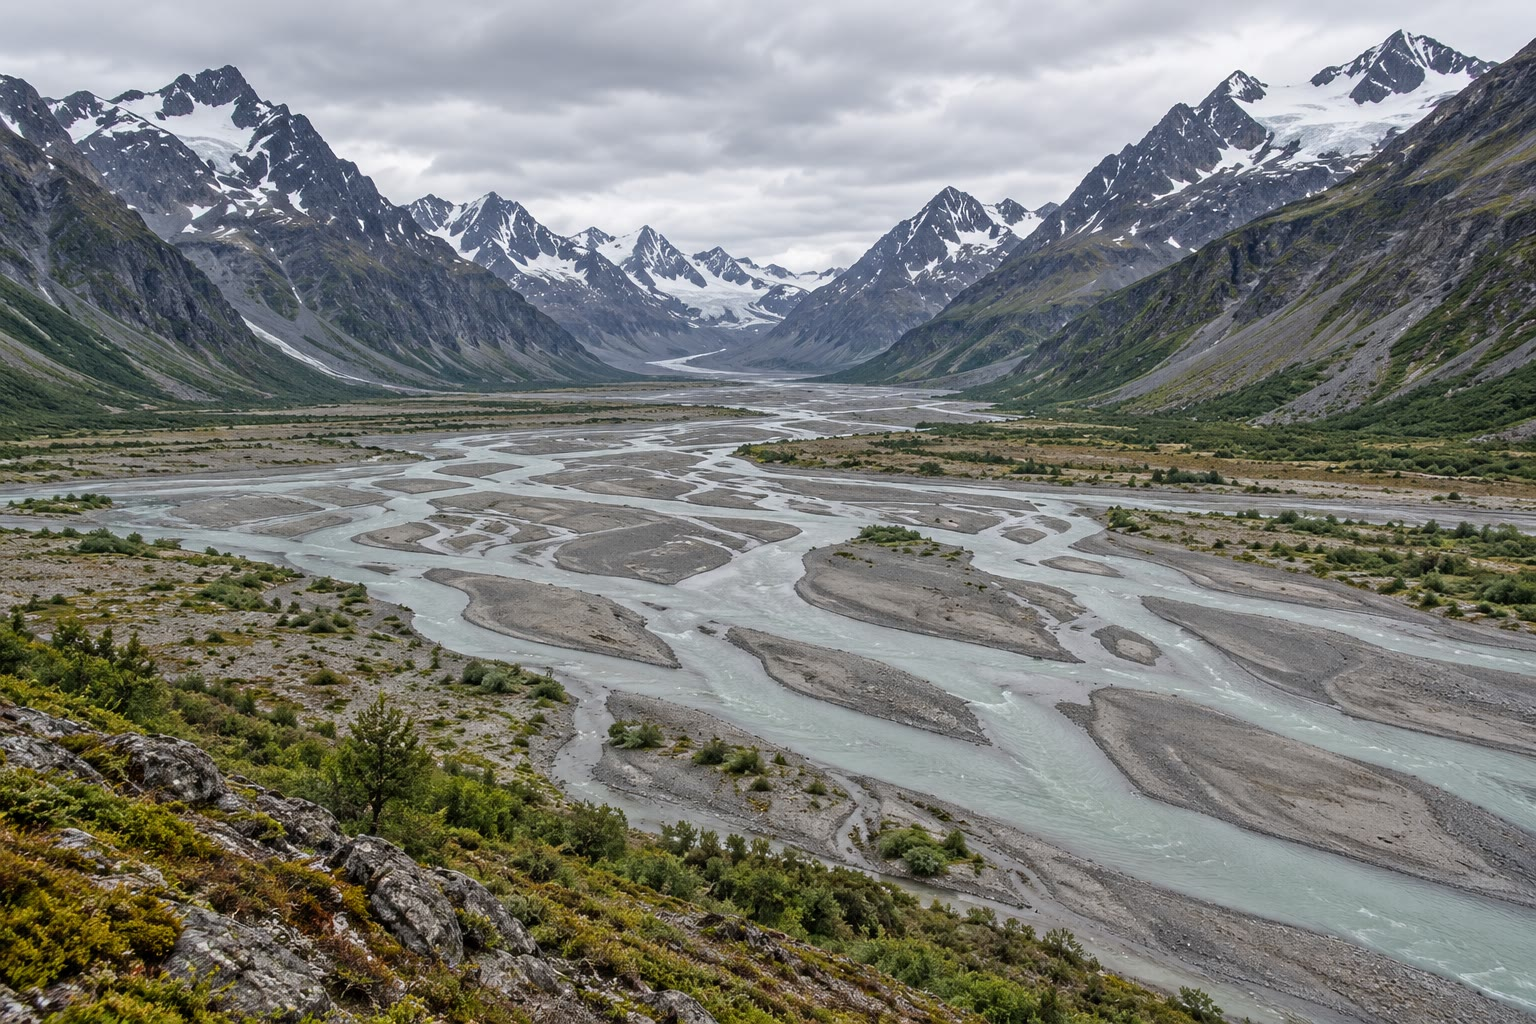
\includegraphics[width=0.66\linewidth]{images/book2/ai/g12-braided-river.jpg}

{\small हिमनदीय पर्वत-घाटी में एक गुंफित नदी: उथली धाराएँ बजरी के उन
टीलों के बीच बँटती और फिर मिलती हैं जिन्हें जल केवल बाढ़ में हिलाता है।
एआई-जनित चित्रण।}
\end{omfigure}

कोई नदी जो ढोती है, उसे मापना \omterm{def:g12:destruction-of-mountains:denudation}{अनाच्छादन दर} ज्ञात करने का एक दूसरा तरीक़ा देता है।

\begin{method}[अपरदन-लेखा]\label{met:g12:destruction-of-mountains:budget}
\begin{enumerate}
  \item वह अवसाद-द्रव्यमान लीजिए जिसे नदी एक वर्ष में ढोती है, और उसमें
        \omterm{def:g12:destruction-of-mountains:load}{घुलित भार} जोड़िए (यदि केवल ठोस भार ज्ञात है, तो उसे
        $0.85$ से भाग दीजिए)।
  \item चट्टान के घनत्व से भाग दीजिए, \omterm{def:g12:continental-crust:continental-crust}{महाद्वीपीय भूपर्पटी} के लिए लगभग \qty{2830}{kg/m^3},
        जिससे हर वर्ष हटाई गई चट्टान का आयतन मिले।
  \item \omterm{def:g10:drainage-basins:drainage-basin}{अपवाह द्रोणी} के क्षेत्रफल से भाग दीजिए: यह हर वर्ष हटाई गई
        मोटाई है।
  \item इसे मीटर प्रति मिलियन वर्ष में व्यक्त करने के लिए $10^6$ से गुणा कीजिए।
\end{enumerate}
\end{method}
% ledger: earle:loads, cm95:crust

\begin{example}[मिसिसिपी]\label{ex:g12:destruction-of-mountains:mississippi}
1900 से पहले मिसूरी--मिसिसिपी नदी-तंत्र लगभग
\qty{2980000}{km^2} की द्रोणी से प्रति वर्ष लगभग 400 मिलियन टन अवसाद समुद्र तक ले जाता था।
\omterm{def:g12:destruction-of-mountains:load}{घुलित भार} के साथ, $400/0.85 \approx 471$ मिलियन
टन, यानी प्रति वर्ष $\num{4.71e11}/2830 \approx \qty{1.66e8}{m^3}$ चट्टान।
$\qty{2.98e12}{m^2}$ पर फैलाने पर यह इतनी मोटी परत है:
\[
  \frac{\num{1.66e8}}{\num{2.98e12}} \approx \qty{5.6e-5}{m}
  \text{ प्रति वर्ष, लगभग } \qty{56}{m/Myr}.
\]
1987 और 2006 के बीच नदी प्रति वर्ष केवल 145 मिलियन टन ले गई, जिससे
लगभग \qty{20}{m/Myr} मिलता है: 1950 के दशक में मिसूरी पर बने बाँध
प्रति वर्ष लगभग 100 से 150 मिलियन टन रोक लेते हैं, और दूसरे निर्माण और भी रोकते हैं।
\end{example}
% ledger: mm10:mississippi, kammerer:mississippi, earle:loads, cm95:crust
% values: miss_before_1900_m_per_myr 55.8, miss_1987_2006_m_per_myr 20.2 (relief_decay.py)

यही लेखा पूरे संसार के लिए बनाया जा सकता है। मनुष्यों द्वारा नदियों को बदलने से
पहले वे प्रति वर्ष लगभग 15.5 अरब टन ठोस अवसाद तटों तक ले जाती थीं;
\omterm{def:g12:destruction-of-mountains:load}{घुलित भार} के साथ, यह प्रति वर्ष लगभग \qty{6.4}{km^3} चट्टान है,
महाद्वीपों के \qty{1.48e8}{km^2} से ली गई: लगभग \qty{43}{m/Myr} की
माध्य \omterm{def:g12:destruction-of-mountains:denudation}{अनाच्छादन दर}, बेरिलियम-10 मापनों की माध्यिका के निकट।
तब से मनुष्यों ने दोनों पद बदल दिए हैं: मृदा-अपरदन ने नदियों द्वारा उठाए जाने वाले भार को
प्रति वर्ष लगभग 2.3 अरब टन बढ़ा दिया है, पर
100 अरब टन से अधिक अवसाद अब बाँधों के पीछे पड़ा है।
% ledger: syvitski:modern-flux (Book 1 row, prehuman 15.5 Gt/yr with bed load), sy05:humans, data:etopo1 (land fraction 0.290, grade-11 hypsometry), cm95:crust
% values: world_volume_km3_per_yr 6.44, land_area_km2 1.48e8, world_m_per_myr 43.5 (relief_decay.py)

\section{अवसाद से चट्टान तक}

नदियाँ जो ढोती हैं, वह वहाँ बिछ जाता है जहाँ धारा धीमी होती है: घाटियों और
झीलों में, डेल्टाओं पर, और सबसे बढ़कर महाद्वीपीय सीमांतों की \omterm{def:g11:fossil-fuel-geology:basin}{अवसादी द्रोणियों} में।
परत-दर-परत अवसाद दबता जाता है, और धीरे-धीरे
चट्टान बन जाता है।

\begin{definition}[खंडज चट्टान; डायजेनेसिस]\label{def:g12:destruction-of-mountains:diagenesis}
\emph{खंडज चट्टान}\index{खंडज चट्टान} (या क्लास्टिक चट्टान)
पुरानी चट्टानों और खनिजों के टुकड़ों, खंडों, से बनी एक अवसादी चट्टान है।
\emph{डायजेनेसिस}\index{डायजेनेसिस} उन परिवर्तनों का समूह है जो किसी दबे हुए
अवसाद को निम्न तापमान पर चट्टान में बदलते हैं: \emph{संहनन}, जब
ऊपर की परतों का भार जल और वायु को निचोड़ बाहर करता है, फिर \emph{सीमेंटन}, जब
छिद्रों के जल से क्रिस्टलित होने वाले खनिज (कैल्साइट, क्वार्ट्ज़,
हेमेटाइट, \omterm{def:g10:soil-formation:clay}{मृत्तिका खनिज}) कणों को आपस में चिपका देते हैं।
\end{definition}
% ledger: earle:clastic

\omterm{def:g12:destruction-of-mountains:diagenesis}{खंडज चट्टानों} के नाम उनके खंडों के आकार से रखे जाते हैं:
\begin{itemize}
  \item \textbf{संगुटिकाश्म} \qty{2}{mm} से बड़े गोल खंडों से बना होता है,
        \textbf{संकोणाश्म} कोणीय खंडों से;
  \item \textbf{बलुआ पत्थर} रेत से बना होता है, \qty{2}{mm}
        और \qty{0.063}{mm} के बीच के कण, अक्सर क्वार्ट्ज़ के, वह खनिज जो अपक्षय का
        सबसे अच्छा प्रतिरोध करता है;
  \item \textbf{पंकाश्म} में कम से कम \qty{75}{\percent} गाद और मृत्तिका होती है;
        यदि वह पतली परतों में फटे, तो वह शेल है।
\end{itemize}
% ledger: earle:clastic

\begin{omfigure}
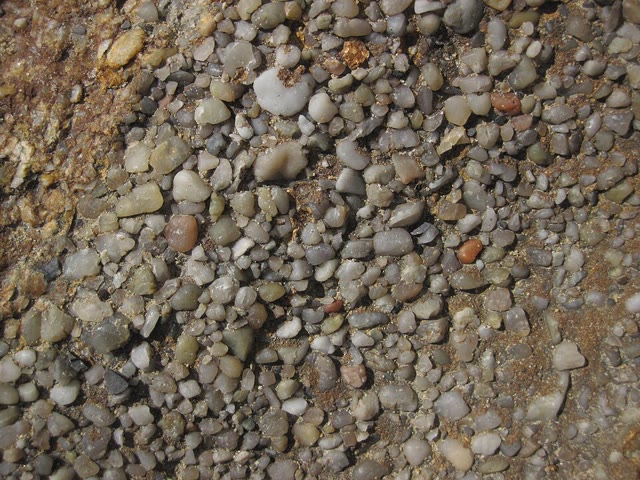
\includegraphics[width=0.5\linewidth]{images/book2/g12-stjohn-conglomerate.jpg}

{\small ओहायो का क्वार्ट्ज़-कंकड़ संगुटिकाश्म, कार्बोनिफ़ेरस आयु का:
क्वार्ट्ज़ के गोल कंकड़, बारीक रेत से सीमेंटित। फ़ोटो जेम्स
सेंट~जॉन (CC~BY~2.0)।}
\end{omfigure}
% ledger: photo:g12-conglomerate, ics:base.Carboniferous, ics:base.Permian (Lower Pennsylvanian lies in the Carboniferous)

खंड यात्रा को दर्ज करते हैं। गोल कंकड़ किसी नदी में या किसी समुद्र-तट पर
लंबी दूरी तक लुढ़के हैं; कोणीय कंकड़ों ने शायद ही यात्रा की हो। लगभग केवल क्वार्ट्ज़
से बना बलुआ पत्थर ऐसी चट्टान से आता है जिसका लंबे समय तक अपक्षय हुआ,
जब तक दूसरे खनिज मृत्तिका में नहीं बदल गए।
% ledger: earle:clastic (rounded/angular, most sand grains quartz, the most resistant mineral)

\section{मूल ऊपर उठता है}

यदि अपरदन केवल किसी श्रेणी के शीर्ष से चट्टान हटाता, तो \qty{2}{km}
ऊँची श्रेणी, \qty{200}{m/Myr} की दर से घिसकर, दस मिलियन वर्षों में समाप्त हो जाती।
पर श्रेणी प्रावार पर तैरती है। जैसे-जैसे शीर्ष से चट्टान हटती है,
स्तंभ हल्का होता जाता है, और ऊपर उठता है।

\begin{definition}[समस्थितिक प्रतिक्षेप]\label{def:g12:destruction-of-mountains:rebound}
\emph{समस्थितिक प्रतिक्षेप}\index{समस्थितिक प्रतिक्षेप} \omterm{def:g11:lithosphere-asthenosphere:lithosphere}{स्थलमंडल} के किसी क्षेत्र का
ऊपर उठना है जब उससे कोई भार हटाया जाता है --- अपरदन से घिसी चट्टान,
या पिघलती हिमचादर --- जब तक \omterm{def:g11:lithosphere-asthenosphere:isostasy}{समस्थिति} फिर से स्थापित न हो जाए।
\end{definition}
% ledger: sella07:gia (rebound after ice unloading)

\begin{proposition}[अपरदन और प्रतिक्षेप]\label{prop:g12:destruction-of-mountains:rebound}
एयरी के मॉडल में, जब अपरदन भूपर्पटी की मोटाई $e$ हटाता है, जिस भूपर्पटी का घनत्व
$\rho_c$ है और जो घनत्व $\rho_m$ वाले प्रावार पर \omterm{def:g11:lithosphere-asthenosphere:isostasy}{समस्थिति} में है, तो
सतह केवल इतनी नीचे जाती है:
\[
  \Delta h = e\left(1 - \frac{\rho_c}{\rho_m}\right),
\]
जबकि भूपर्पटी का आधार $e\,\rho_c/\rho_m$ ऊपर उठता है।
\end{proposition}

\begin{proof}
शीर्ष से $e$ हटाने पर भूपर्पटी $e$ पतली हो जाती है। एयरी के मॉडल से,
$e$ पतली भूपर्पटी $e\,(\rho_m - \rho_c)/\rho_m = e(1 -
\rho_c/\rho_m)$ नीचे खड़ी होती है। भूपर्पटी का शीर्ष इतना नीचे गया है, और उसकी
मोटाई $e$ घटी है, इसलिए उसका आधार $e - e(1 -
\rho_c/\rho_m) = e\,\rho_c/\rho_m$ ऊपर उठा है।
\end{proof}

$\rho_c = \qty{2830}{kg/m^3}$ और $\rho_m = \qty{3380}{kg/m^3}$ के साथ $1 -
\rho_c/\rho_m \approx 0.163$। \qty{1}{km} चट्टान हटाने से
सतह केवल लगभग \qty{163}{m} नीचे जाती है: बाक़ी \qty{837}{m} की पूर्ति
पूरे स्तंभ के ऊपर उठने से होती है। किसी श्रेणी को \qty{2000}{m} नीचे करने के लिए अपरदन को
लगभग $2000/0.163 \approx \qty{12300}{m}$ चट्टान हटानी पड़ती है। जो चट्टानें
\qty{12}{km} से अधिक नीचे थीं, श्रेणी की गहराइयों में बनी कायांतरित चट्टानें और ग्रेनाइट,
सतह पर पहुँच जाती हैं: इसीलिए पुरानी, घिसी हुई पर्वत-पट्टियाँ
विशाल क्षेत्रों में शिस्ट, नाइस और ग्रेनाइट अनावृत करती हैं।
% ledger: cm95:crust, data:prem (rho 3.38 below the Moho)
% values: rebound_fraction 0.16272, lowering_per_km_m 162.7, root_rise_per_km_m 837.3, eroded_for_2000m_km 12.29 (relief_decay.py)

\begin{omfigure}
\begin{tikzpicture}[x=1cm, y=1cm, font=\scriptsize]
  % three columns: before, after erosion without rebound, after rebound
  \foreach \i/\top/\base/\lab in {0/3.0/-3.2/{समस्थिति में एक श्रेणी}, 1/2.0/-3.2/{अपरदन $e$ हटाता है}, 2/2.84/-2.36/{स्तंभ ऊपर उठता है}} {
    \begin{scope}[xshift=\i*4.6cm]
      \fill[omLithPeridotite!45] (0,-3.6) rectangle (3.4,-0.6);
      \fill[omLithGranite!55, draw=black!60] (0.5,\base) -- (0.5,0) -- (1.0,\top) -- (2.4,\top) -- (2.9,0) -- (2.9,\base) -- cycle;
      \fill[omLithGranite!55, draw=black!60] (0,0) rectangle (0.5,-0.6);
      \fill[omLithGranite!55, draw=black!60] (2.9,0) rectangle (3.4,-0.6);
      \draw[black!40, densely dashed] (-0.1,0) -- (3.5,0);
      \node[anchor=north, align=center, text width=3.4cm] at (1.7,-3.75) {\lab};
    \end{scope}
  }
  % eroded slab, middle panel
  \draw[omThm, densely dashed] (4.6+1.0,3.0) -- (4.6+2.4,3.0);
  \draw[omThm, |-|] (4.6+2.65,3.0) -- node[right] {$e$} (4.6+2.65,2.0);
  % right panel: the old top and base
  \draw[omThm, densely dashed] (9.2+1.0,3.0) -- (9.2+2.4,3.0);
  \draw[omThm, densely dashed] (9.2+0.5,-3.2) -- (9.2+2.9,-3.2);
  \draw[-{Stealth}, omDef, line width=0.9pt] (9.2+1.7,-3.15) -- (9.2+1.7,-2.45);
  \node[omDef, anchor=west] at (9.2+3.0,-2.8) {मूल ऊपर उठता है};
  \node[anchor=west] at (9.2+3.0,2.95) {सतह केवल};
  \node[anchor=west] at (9.2+3.0,2.55) {$0.16\,e$ नीचे};
  \draw[black!60, |-|] (9.2+2.65,3.0) -- (9.2+2.65,2.84);
  % labels
  \node[anchor=west] at (3.45,-2.1) {प्रावार};
  \node at (1.7,-1.5) {भूपर्पटी};
\end{tikzpicture}

{\small अपरदन और \omterm{def:g12:destruction-of-mountains:rebound}{समस्थितिक प्रतिक्षेप} (योजनाबद्ध, ऊँचाइयाँ पैमाने पर नहीं)। बाएँ:
\omterm{def:g11:lithosphere-asthenosphere:isostasy}{समस्थिति} में एक श्रेणी, अपने \omterm{def:g12:continental-crust:root}{मूल} के साथ। बीच में: अपरदन शीर्ष से मोटाई $e$
हटाता है। दाएँ: हल्का स्तंभ तब तक ऊपर उठता है जब तक \omterm{def:g11:lithosphere-asthenosphere:isostasy}{समस्थिति} फिर से स्थापित न हो जाए;
सतह अंत में शुरुआत से केवल $0.163\,e$ नीचे रहती है, और \omterm{def:g12:continental-crust:root}{मूल}
$0.837\,e$ ऊपर उठ चुका है।}
\end{omfigure}

यही प्रतिक्षेप आज वहाँ देखा जा सकता है जहाँ कोई भार जल्दी लुप्त हुआ।
अंतिम हिमनदीय अधिकतम पर कनाडा के बड़े भाग को ढकने वाली हिमचादर
हडसन खाड़ी के आसपास सबसे मोटी थी। वह बर्फ़ पिघल चुकी है, और वहाँ भूमि अब भी
उठ रही है: GPS से मापी गई, प्रति वर्ष लगभग \qty{10}{mm}, यानी
\qty{10000}{m/Myr}, \omterm{def:g10:drainage-basins:drainage-basin}{अपवाह द्रोणियों} की माध्य \omterm{def:g12:destruction-of-mountains:denudation}{अनाच्छादन दर} का लगभग पचास
गुना। और दक्षिण में,
महान झीलों के पार, भूमि प्रति वर्ष 1 से \qty{2}{mm} धँसती है।
% ledger: sella07:gia, pb11:rates

\section{कोई श्रेणी कितने समय टिकती है?}

कोई द्रोणी जितनी खड़ी, वह उतनी ही तेज़ी से अपरदित होती है; बड़ी द्रोणियों के लिए \omterm{def:g12:destruction-of-mountains:denudation}{अनाच्छादन
दर} उनकी माध्य उच्चावच के समानुपाती पाई गई है। आइए वह
सबसे सरल मॉडल लें जो यही कहता है।

\begin{proposition}[किसी श्रेणी का चरघातांकी क्षय]\label{prop:g12:destruction-of-mountains:decay}
मान लीजिए $h(t)$ किसी श्रेणी की उसके चारों ओर के मैदानों से ऊपर माध्य ऊँचाई है। यदि
\omterm{def:g12:destruction-of-mountains:denudation}{अनाच्छादन दर} $E = k\,h$ है, जहाँ $k$ एक स्थिरांक है, और यदि \omterm{def:g11:lithosphere-asthenosphere:isostasy}{समस्थिति} हर समय
बहाल रहती है, तो
\[
  h(t) = h_0\, e^{-f k t}, \qquad f = 1 - \frac{\rho_c}{\rho_m},
\]
जहाँ $h_0$, $t = 0$ पर की ऊँचाई है। ऊँचाई $e$ से विभाजित हो जाती है,
हर $\tau = 1/(fk)$ में, और दो से, हर $\tau \ln 2$ में।
\end{proposition}

\begin{proof}
एक छोटे समय $\mathrm{d}t$ में अपरदन $E\,\mathrm{d}t
= k h\,\mathrm{d}t$ मोटाई हटाता है, और पिछले प्रस्ताव से सतह
$f k h\,\mathrm{d}t$ नीचे जाती है। इसलिए $h' = -fk\,h$, और इस
समीकरण के हल $h(t) = h_0\,e^{-fkt}$ हैं। $t = \tau$ पर $h = h_0/e$; $h = h_0/2$
तब, जब $fkt = \ln 2$।
\end{proof}

बड़ी द्रोणियों पर मापन $k$ देते हैं: बिना किसी उत्थान के, उनकी उच्चावच
लगभग 11 मिलियन वर्षों में दसवें भाग तक गिर जाती। इसलिए $e^{-11k} = 0.1$, और $k =
\ln 10/11 \approx 0.209$ प्रति मिलियन वर्ष। प्रतिक्षेप के बिना ($f = 1$)
काल-स्थिरांक $1/k \approx 4.8$ मिलियन वर्ष होता। प्रतिक्षेप के साथ, $f
\approx 0.163$ और
\[
  \tau = \frac{1}{0.163 \times 0.209} \approx 29 \text{ मिलियन वर्ष},
\]
और माध्य ऊँचाई हर $29 \ln 2 \approx 20$ मिलियन वर्षों में आधी हो जाती है:
प्रतिक्षेप किसी श्रेणी को लगभग छह गुना अधिक टिकाता है।
% ledger: ahnert70:decay, cm95:crust, data:prem
% values: k_per_myr 0.20933, tau_none_myr 4.777, tau_rebound_myr 29.36, half_rebound_myr 20.35, half_none_myr 3.31 (relief_decay.py)

\begin{omfigure}
\begin{tikzpicture}
\begin{axis}[omrecord, width=0.7\linewidth, height=5.4cm, xmin=0, xmax=100, ymin=0, ymax=2100,
  xlabel={समय (मिलियन वर्ष)}, ylabel={माध्य ऊँचाई (\unit{m})},
  xtick={0,20,...,100}, ytick={0,500,...,2000}]
% computed in figdata/grade-12/relief_decay.py; ledger: ahnert70:decay, cm95:crust, data:prem
\addplot[omProp, line width=1.1pt, densely dashed] table[x=t_Myr, y=h_none] {figdata/out/grade-12-relief_decay-curve.dat};
\addplot[omDef, line width=1.1pt] table[x=t_Myr, y=h_rebound] {figdata/out/grade-12-relief_decay-curve.dat};
\draw[black!45, densely dotted] (axis cs:20.35,0) -- (axis cs:20.35,1000) -- (axis cs:0,1000);
\draw[omProp, line width=0.4pt] (axis cs:9,304) -- (axis cs:33,215);
\coordinate (none) at (axis cs:33.5,215);
\coordinate (reb) at (axis cs:45,780);
\end{axis}
\node[font=\scriptsize, text=omProp, anchor=west] at (none) {प्रतिक्षेप के बिना};
\node[font=\scriptsize, text=omDef, anchor=south west] at (reb) {प्रतिक्षेप के साथ};
\end{tikzpicture}

{\small \qty{2000}{m} ऊँची किसी श्रेणी की माध्य ऊँचाई, जो अपनी ऊँचाई के समानुपाती दर से
घिसती है, \omterm{def:g12:destruction-of-mountains:rebound}{समस्थितिक प्रतिक्षेप} के साथ और उसके बिना; प्रतिक्षेप के
साथ, 20 मिलियन वर्षों के बाद आधी ऊँचाई बचती है (बिंदुकित)। दर-स्थिरांक
एनर्ट (1970) से; भूपर्पटी और \omterm{def:g11:seismic-structure:moho}{मोहो} के नीचे के प्रावार के
घनत्व।}
\end{omfigure}

ऐपलेशियन इस चित्र की परीक्षा लेते हैं। उनकी टक्कर पर्मियन में,
250 मिलियन वर्ष से भी पहले, समाप्त हुई। यह उस समय के बारह गुने से भी अधिक है जो
मॉडल ऊँचाई को आधा करने में लेता है: $2000 \times e^{-250/29} \approx
\qty{0.4}{m}$। फिर भी माउंट मिचेल अब भी समुद्र से \qty{2037}{m} ऊपर उठा है।
अकेला मॉडल वर्तमान उच्चावच की व्याख्या नहीं कर सकता: तब से इस प्रदेश को
फिर से ऊपर उठाया गया होगा, या वह मॉडल की धारणा से धीमे अपरदित हुआ होगा।
% ledger: usgs:alleghanian, usgs:alleghanian-age, ics:base.Triassic, ncparks:mitchell, ahnert70:decay
% values: h_after_250myr_rebound_m 0.40 (relief_decay.py)

इस तरह पर्वतों का पुनर्चक्रण होता है। किसी श्रेणी से घिसी चट्टान \omterm{def:g11:fossil-fuel-geology:basin}{अवसादी
द्रोणियों} में पहुँचती है, जहाँ वह \omterm{def:g12:destruction-of-mountains:diagenesis}{खंडज चट्टान} बनती है; उस चट्टान का कुछ भाग इतना गहरा
दबता है कि कायांतरित हो जाए या पिघल भी जाए, कुछ किसी \omterm{def:g11:subduction-zones:subduction}{क्षेपण क्षेत्र} पर प्रावार में
ले जाया जाता है (\cref{ch:g12:subduction-magmatism}), और कुछ
दो महाद्वीपों के टकराने पर फिर से मुड़कर एक नई श्रेणी बन जाता है।
% ledger: ss09:balance (sediment subducted), earle:collision (sediments of both margins in the mountains)

\begin{omfigure}
\begin{tikzpicture}
\begin{axis}[omsection, x=1.25cm, y=0.003125cm, xmin=0, xmax=9.49, ymin=-700, ymax=650,
  xlabel={A से दूरी (\unit{km})}, ylabel={ऊँचाई (\unit{m})},
  ytick={-600,-300,0,300,600}, tick label style={font=\scriptsize}, unbounded coords=jump]
% shared region tables (figdata/shared/region.py); unconformity from figdata/grade-12/relief_decay.py; ledger: region:name
\addplot[fill=black!8, draw=black!50, line width=0.3pt, even odd rule] table {figdata/out/shared-region-section-unit-schist.dat};
\addplot[fill=icsTriassic!20, draw=black!50, line width=0.3pt, even odd rule] table {figdata/out/shared-region-section-unit-sandstone.dat};
\addplot[fill=icsJurassic!25, draw=black!50, line width=0.3pt, even odd rule] table {figdata/out/shared-region-section-unit-limestone.dat};
\addplot[fill=icsJurassic!8, draw=black!50, line width=0.3pt, even odd rule] table {figdata/out/shared-region-section-unit-shale.dat};
\addplot[fill=icsCretaceous!20, draw=black!50, line width=0.3pt, even odd rule] table {figdata/out/shared-region-section-unit-chalk.dat};
\addplot[fill=omLithAlluv, draw=black!50, line width=0.3pt, even odd rule] table {figdata/out/shared-region-section-unit-alluvium.dat};
\addplot[black, line width=0.7pt] table {figdata/out/shared-region-section-ground.dat};
\addplot[omThm, line width=1.4pt] table[x=s_km, y=z_m] {figdata/out/grade-12-relief_decay-unconformity.dat};
\addplot[fault] table {figdata/out/shared-region-section-fault.dat};
\node[anchor=south east, font=\small\bfseries] at (axis cs:0,650) {A};
\node[anchor=south west, font=\small\bfseries] at (axis cs:9.49,650) {B};
\node[font=\scriptsize, fill=white, inner sep=1pt] at (axis cs:1.2,-520) {शिस्ट, लगभग 480 Ma};
\coordinate (unc) at (axis cs:1.6,-300);
\end{axis}
\node[font=\scriptsize, text=omThm, anchor=west, fill=white, inner sep=1pt] at ([xshift=4pt]unc) {विषमविन्यास};
\end{tikzpicture}

\smallskip
{\small\tikz\fill[black!8, draw=black!50] (0,0) rectangle (0.35,0.22);~शिस्ट \quad
\tikz\fill[icsTriassic!20, draw=black!50] (0,0) rectangle (0.35,0.22);~बलुआ पत्थर (ट्राइऐसिक) \quad
\tikz\fill[icsJurassic!25, draw=black!50] (0,0) rectangle (0.35,0.22);~चूना पत्थर \quad
\tikz\fill[icsJurassic!8, draw=black!50] (0,0) rectangle (0.35,0.22);~शेल \quad
\tikz\fill[icsCretaceous!20, draw=black!50] (0,0) rectangle (0.35,0.22);~खड़िया \quad
\omve{2.5}}

{\small वार्डन पहाड़ियों के आर-पार काट A--B, विषमविन्यास लाल में:
वह समतल आधार जिस पर ट्राइऐसिक बलुआ पत्थर शिस्ट के आधार-शैल के आर-पार
बिछाया गया, बाद में मुड़ा और भ्रंशित हुआ। आँकड़े: श्रृंखला का क्षेत्र-मॉडल।}
\end{omfigure}
% values: unconformity sampled from region.contact_elevation('sandstone'); varden_gap_myr 58.1 (relief_decay.py)

वार्डन पहाड़ियाँ ऐसे एक चक्र का अभिलेख रखती हैं। उनका आधार-शैल एक शिस्ट है,
जो लगभग 480 मिलियन वर्ष पहले कायांतरित हुआ, और जिसमें लगभग 310 मिलियन वर्ष पहले
एक ग्रेनाइट अंतर्वेधित हुआ --- दोनों किसी पुरानी पर्वत-पट्टी की सतह से किलोमीटरों नीचे
बने। फिर भी लगभग 252
मिलियन वर्ष पहले से बिछाया गया ट्राइऐसिक बलुआ पत्थर सीधे उन पर, एक समतल सतह के आर-पार, टिका है:
विषमविन्यास। 60 मिलियन वर्ष से कम में वह पुरानी श्रेणी घिसकर
एक मैदान बन चुकी थी और उसकी गहरी चट्टानें सतह पर आ चुकी थीं। फिर समुद्र
उस मैदान पर फैला और उसे दबा दिया।
% ledger: region:name (model: schist 480 Ma, granite 310 Ma, erosion, unconformity, Triassic cover), ics:base.Triassic
% values: varden_gap_myr 58.1 (relief_decay.py)

\section{अभ्यास}

\begin{exercise}[$\star$]\label{exo:g12:destruction-of-mountains:1}
शब्द बताइए: (a) किसी क्षेत्र से प्रति इकाई समय हटाई गई चट्टान की माध्य
मोटाई; (b) वे कण जिन्हें नदी अपनी तली के अनुदिश लुढ़काती और उछालती है; (c) वे
आयन जिन्हें नदी विलयन में ढोती है; (d) वे परिवर्तन जो किसी दबे अवसाद को
चट्टान में बदलते हैं; (e) \omterm{def:g11:lithosphere-asthenosphere:lithosphere}{स्थलमंडल} का ऊपर उठना जब उससे कोई भार हटाया जाता है।
\end{exercise}

\begin{exercise}[$\star$]\label{exo:g12:destruction-of-mountains:2}
\omterm{def:g12:destruction-of-mountains:diagenesis}{खंडज चट्टान} का नाम बताइए: (1) आपस में सीमेंटित \qtyrange{5}{20}{mm} के गोल
कंकड़; (2) \qty{0.3}{mm} के क्वार्ट्ज़ कण; (3) एक चट्टान जो
\qty{90}{\percent} गाद और मृत्तिका है और पतली पट्टियों में फटती है; (4) \qty{3}{cm} के
कोणीय टुकड़े।
\end{exercise}

\begin{exercise}[$\star$]\label{exo:g12:destruction-of-mountains:3}
मिलीमीटर प्रति वर्ष में बदलिए: (1) \qty{54}{m/Myr}; (2) \qty{218}{m/Myr};
(3) हडसन खाड़ी के निकट प्रति वर्ष \qty{10}{mm} का उत्थान, \unit{m/Myr} में।
\end{exercise}

\begin{exercise}[$\star$]\label{exo:g12:destruction-of-mountains:4}
एक नदी प्रति वर्ष 60 मिलियन टन ठोस अवसाद ढोती है। यह जानकर कि \omterm{def:g12:destruction-of-mountains:load}{घुलित भार}
औसतन ढोए गए कुल द्रव्यमान का \qty{15}{\percent} होता है,
उसके \omterm{def:g12:destruction-of-mountains:load}{घुलित भार} का अनुमान लगाइए।
\end{exercise}

\begin{exercise}[$\star$]\label{exo:g12:destruction-of-mountains:5}
सतह से नीचे की ओर क्रम में रखिए कि किसी ग्रेनाइट के क्वार्ट्ज़ के एक कण के साथ
क्या होता है: किसी द्रोणी में निक्षेपण, ग्रेनाइट का अपक्षय,
नई परतों के नीचे दबना, किसी नदी द्वारा परिवहन, सीमेंटन।
\end{exercise}

\begin{exercise}[$\star\star$]\label{exo:g12:destruction-of-mountains:6}
एक धारा \qty{30}{cm/s} से धीमी होकर \qty{5}{cm/s} हो जाती है। अध्याय के मानों का
उपयोग करके बताइए कि तली पर पड़े \qty{1}{mm} के रेत-कण का, और
पहले से निलंबन में \qty{0.01}{mm} के गाद-कण का, हर चाल पर
क्या होता है।
\end{exercise}

\begin{exercise}[$\star\star$]\label{exo:g12:destruction-of-mountains:7}
\qty{50000}{km^2} की एक द्रोणी प्रति वर्ष 4 मिलियन टन ठोस अवसाद समुद्र को भेजती है।
\omterm{def:g12:destruction-of-mountains:load}{घुलित भार} सहित उसका अपरदन-लेखा बनाइए, $\rho =
\qty{2830}{kg/m^3}$ के साथ। बेरिलियम-10 द्रोणी-दरों की माध्यिका से तुलना कीजिए।
\end{exercise}

\begin{exercise}[$\star\star$]\label{exo:g12:destruction-of-mountains:8}
(1) $1 - \rho_c/\rho_m$ परिकलित कीजिए, जहाँ $\rho_c = \qty{2700}{kg/m^3}$ और
$\rho_m = \qty{3300}{kg/m^3}$। (2) \qty{1}{km} चट्टान
अपरदित होने पर सतह कितनी नीचे जाती है? (3) अध्याय के मान से तुलना कीजिए।
\end{exercise}

\begin{exercise}[$\star\star$]\label{exo:g12:destruction-of-mountains:9}
एक ग्रेनाइट किसी श्रेणी के नीचे लगभग \qty{8}{km} की गहराई पर क्रिस्टलित हुआ। (1) उसे सतह पर
लाने के लिए अपरदन को कितनी मोटी चट्टान हटानी होगी? (2) इस बीच माध्य सतह
कितनी नीचे जाती है? (3) \qty{200}{m/Myr} पर
इसमें कितना समय लगता है?
\end{exercise}

\begin{exercise}[$\star\star$]\label{exo:g12:destruction-of-mountains:10}
महाद्वीपों की माध्य ऊँचाई लगभग \qty{794}{m} है। (1)
\qty{43}{m/Myr} पर अपरदन को इतनी मोटी परत हटाने में कितना समय लगेगा?
(2) यदि \omterm{def:g12:destruction-of-mountains:rebound}{समस्थितिक प्रतिक्षेप} को ध्यान में रखा जाए और दर वही रहे, तो कितना?
(3) फिर भी 4 अरब वर्षों के बाद महाद्वीप अब भी समुद्र से ऊपर क्यों
खड़े हैं?
\end{exercise}

\begin{exercise}[$\star\star$]\label{exo:g12:destruction-of-mountains:11}
ज़्यादातर पिछले पचास वर्षों में बने बाँधों के पीछे 100 अरब टन से अधिक अवसाद
पड़ा है। (1) \qty{2830}{kg/m^3} पर यह चट्टान का कितना आयतन है?
(2) यह संसार के मानव-पूर्व ठोस भार, प्रति वर्ष 15.5 अरब टन,
के कितने वर्षों के बराबर है?
\end{exercise}

\begin{exercise}[$\star\star\star$]\label{exo:g12:destruction-of-mountains:12}
दिखाइए कि अध्याय के मॉडल में किसी श्रेणी की \omterm{def:g12:destruction-of-mountains:denudation}{अनाच्छादन दर}
$E(t) = k h_0 e^{-fkt}$ है। माध्य ऊँचाई के $h_0$ से 0 तक गिरने के दौरान
हटाई गई चट्टान की कुल मोटाई परिकलित कीजिए, और परिणाम को
प्रतिक्षेप वाले प्रस्ताव से समझाइए।
\end{exercise}

\begin{exercise}[$\star\star\star$]\label{exo:g12:destruction-of-mountains:13}
हडसन खाड़ी के निकट भूमि प्रति वर्ष \qty{10}{mm} उठती है। (1) यदि वह दर
वही रहे, तो वह 1000 वर्षों में कितनी उठेगी? (2) यह उठान किसी हिमचादर के पिघलने के बाद का
प्रतिक्षेप है। बर्फ़ का घनत्व
\qty{900}{kg/m^3} और प्रावार का \qty{3380}{kg/m^3} लीजिए: एयरी के मॉडल में
\qty{2}{km} बर्फ़ पिघलने के बाद भूमि कुल मिलाकर कितनी उठेगी?
(3) समय के साथ दर धीमी क्यों होनी चाहिए?
\end{exercise}
% ledger: sella07:gia, usgs:ice-density (ice about 90 % as dense as water), data:prem

\begin{exercise}[$\star\star\star$]\label{exo:g12:destruction-of-mountains:14}
मिसिसिपी 1900 से पहले प्रति वर्ष 400 मिलियन टन ठोस अवसाद ढोती थी
और 1987--2006 में प्रति वर्ष 145 मिलियन टन। (1) दोनों अवधियों में
उसकी \qty{2980000}{km^2} की द्रोणी की \omterm{def:g12:destruction-of-mountains:denudation}{अनाच्छादन दर}, \omterm{def:g12:destruction-of-mountains:load}{घुलित भार} सहित,
परिकलित कीजिए। (2) दोनों में से कौन-सी द्रोणी के प्राकृतिक अपरदन को बेहतर
मापती है? (3) बाँध प्रति वर्ष 100 से 150 मिलियन टन रोकते हैं: क्या इससे
पूरी कमी की व्याख्या हो जाती है?
\end{exercise}

\begin{exercise}[$\star\star\star$]\label{exo:g12:destruction-of-mountains:15}
वार्डन पहाड़ियों में लगभग 310 मिलियन वर्ष पहले अंतर्वेधित एक ग्रेनाइट
ट्राइऐसिक बलुआ पत्थर के नीचे पड़ा है, जो लगभग 252 मिलियन वर्ष पहले से बिछाया गया।
मान लीजिए ग्रेनाइट \qty{6}{km} नीचे क्रिस्टलित हुआ। (1) उसके ऊपर से कम से कम
कितनी मोटी चट्टान हटाई गई? (2) इसके लिए कम से कम कौन-सी माध्य \omterm{def:g12:destruction-of-mountains:denudation}{अनाच्छादन दर}
आवश्यक है? (3) द्रोणियों की मापी गई दरों से तुलना कीजिए।
\end{exercise}

\begin{problem}[{सप्ताहांत समस्या --- किसी पर्वत-श्रेणी को समतल करने में कितना समय?}]
\label{pb:g12:destruction-of-mountains:1}
% ledger: pb11:rates, ahnert70:decay, cm95:crust, data:prem, usgs:alleghanian, usgs:alleghanian-age, ics:base.Triassic, ncparks:mitchell, photo:g12-appalachians
% values (relief_decay.py): k 0.20933/Myr, E0 418.7 m/Myr, f 0.16272, tau 4.777 / 29.36 Myr, half-lives 3.31 / 20.35 Myr
एक युवा श्रेणी की अपने चारों ओर के मैदानों से ऊपर माध्य ऊँचाई \qty{2000}{m} है।
उसकी नदियाँ उसे उसकी ऊँचाई के समानुपाती दर से घिसती हैं, $E = kh$,
जहाँ $k = 0.209$ प्रति मिलियन वर्ष। भूपर्पटी का घनत्व
\qty{2830}{kg/m^3} है, उसके नीचे के प्रावार का \qty{3380}{kg/m^3}।

\medskip
\noindent\textbf{भाग I --- अपरदन दर।}
\begin{enumerate}
  \item आज श्रेणी की \omterm{def:g12:destruction-of-mountains:denudation}{अनाच्छादन दर} \unit{m/Myr} में परिकलित कीजिए।
  \item इसे मिलीमीटर प्रति वर्ष में व्यक्त कीजिए।
  \item इसकी तुलना भूकंपीय रूप से सक्रिय द्रोणियों
        (\qty{367}{m/Myr}) और शांत द्रोणियों (\qty{182}{m/Myr}) में मापी गई माध्य दरों से कीजिए।
  \item किसी द्रोणी का कौन-सा लक्षण उसकी अपरदन दर का सबसे अच्छा पूर्वानुमान देता है?
  \item श्रेणी के हर वर्ग किलोमीटर से हर वर्ष कितने टन चट्टान
        निकलती है?
\end{enumerate}

\medskip
\noindent\textbf{भाग II --- प्रतिक्षेप के बिना।}
\begin{enumerate}[resume]
  \item यदि दर अपने वर्तमान मान पर रहती, तो \qty{2000}{m} चट्टान हटाने में
        कितना समय लगता?
  \item वास्तव में श्रेणी के नीचे होने के साथ दर घटती है। समीकरण
        $h' = -kh$ और $h(0) = \qty{2000}{m}$ के साथ उसका हल लिखिए।
  \item काल-स्थिरांक $1/k$ क्या है?
  \item ऊँचाई को आधा होने में कितना समय लगता है?
  \item जाँचिए कि 11 मिलियन वर्षों के बाद ऊँचाई का दसवाँ भाग बचता है।
\end{enumerate}

\medskip
\noindent\textbf{भाग III --- प्रतिक्षेप के साथ।}
\begin{enumerate}[resume]
  \item $f = 1 - \rho_c/\rho_m$ परिकलित कीजिए।
  \item जब \qty{100}{m} चट्टान अपरदित होती है, तो सतह कितनी नीचे
        जाती है, और \omterm{def:g12:continental-crust:root}{मूल} कितना ऊपर उठता है?
  \item $h$ का नया समीकरण और उसका हल लिखिए।
  \item श्रेणी को \qty{2000}{m} से \qty{200}{m} तक नीचे लाने के लिए
        कितनी मोटी चट्टान अपरदित होनी चाहिए?
  \item इससे किस प्रकार की चट्टानें सतह पर आती हैं?
\end{enumerate}

\medskip
\noindent\textbf{भाग IV --- काल-स्थिरांक।}
\begin{enumerate}[resume]
  \item प्रतिक्षेप के साथ काल-स्थिरांक परिकलित कीजिए।
  \item श्रेणी को अपनी ऊँचाई के दसवें भाग तक गिरने में कितना समय लगता है?
  \item 200 मिलियन वर्षों के बाद वह कितनी ऊँची है?
  \item ऐपलेशियन टक्कर 250 मिलियन वर्ष से भी पहले समाप्त हुई।
        यदि श्रेणी कभी फिर से ऊपर न उठाई गई होती, तो 250 मिलियन वर्षों के बाद मॉडल उसे
        कितनी ऊँची छोड़ता? माउंट मिचेल अब भी समुद्र से \qty{2037}{m}
        ऊपर उठा है: इससे क्या संकेत मिलता है?
  \item सारांश दीजिए: कितने मिलियन वर्षों में श्रेणी की माध्य ऊँचाई
        आधी होती है?
\end{enumerate}
\end{problem}
